\section{Forecasting COVID-19 time series}


\subsection{Data Selection}
We integrated the user interface for forecasting tightly with the chart analysis feature. They go hand in hand. The user visualizes the time series they are interested in. It follows that they also want to create predictions for exactly that time series. They can create a new model with a button and the data they previously selected is now the input data to train their model. They get to generate a forecast right away by using the default hyper parameters supplied by the system. Should they want to change the data (e.g., select a different time frame), they can easily update the chart and update their model and the forecast.

\subsection{Behind the scenes}
Once the user wants to fit their model to the data, the backend creates a job and adds it to a queue. The prediction engine takes the job and fits the model. It creates a forecast a third into the future of the original time frame length and writes the resulting prediction back into the database. This includes uncertainty intervals. We made the prediction horizon a third of the input data length, to (1) reduce the number of things users have to configure and (2) we don't want a user to be able to create forecasts too far into the future, as those will not be usable and potentially lead to the wrong conclusions.

The prediction engine is a small container running Python that can be scaled horizontally very well as it acts as a worker.

\subsection{Forecasting}

There are common time series features that we care about when creating a forecast. One are seasonal cycles, e.g., a weekly seasonality that shows recurring patterns throughout the weekdays or a yearly seasonality that might show a dip towards the end of the year for example. Another feature are trend changes over time. We might also notice effects of holidays events. And the last feature we can observe are outliers.

The authors of the paper Forecasting at Scale \cite{b1} explain the insufficiency of previous forecasting methods by taking an example time series that they recorded and tried fitting the data in an automated setting without changing the default parameters on these data. The referenced approaches were Autoregressive Integrate Moving Average (ARIMA) \cite{b2}, Exponential Smoothing \cite{b3}, and Trigonometric seasonality, Box-Cox transformation, Autoregressive Moving Average (ARMA) errors, Trend and Seasonal components (TBATS) \cite{b4} as well as an unreferenced naive approach using a random walk making constant predictions with a weekly seasonality.

The result was that these methods can be made to work, if one tweaks their parameters. Figuring out the parameter values can be tricky if the user is not trained in these models. For example, ARIMA has three main parameters (1) maximum order of differencing, (2) autoregressive components, and (3) moving average components. Without proper understanding of these parameters and their effects it is hard to find a good fit.

The authors created an R and Python library that implements the described methods of their paper and named it Prophet\footnote{\href{https://facebook.github.io/prophet/}{https://facebook.github.io/prophet/}}.

\subsection{The Prophet Forecasting Model}

We know the features of a time series. We can model this as separate components that we additively combine to a prediction model. We add the trend \(g(t)\) modeling nonperiodic changes, the seasonality \(s(t)\) modeling the periodic changes, the holidays and events \(h(t)\) modeling single data point effects which are potentially irregular, and the error term \(\epsilon_t\) that is assumed to be normally distributed.


\begin{equation}
    y(t)=g(t)+s(t)+h(t)+\epsilon_t
    \label{eq:fullTrendModel}
\end{equation}


The advantages of this model are 

\begin{itemize}
    \item computationally simple, making fitting it to data very fast
    \item cognitively simple, making it easily interpretable by human analysts
    \item adding new components is easy since we're using addition and no normalization factors need to be introduced
\end{itemize}


The addition aspect of the model however means that we cannot model a trend change that amplifies the effects of the seasonality component as they are assumed to be independent. The authors later made their software Prophet capable of producing forecasts with multiplicative seasonality as well, after the publishing of the paper. We allow users to select which seasonality mode they want to use to train their model. If the magnitude of seasonality effects grows with the time series itself, it could be interesting for the user to use multiplicative seasonality. 

\textbf{Trend:} The mathematical expression to compute the nonlinear, saturating growth trend in its most basic form is the standard trend formula with \(C\) as the carrying capacity, \(k\) as the growth rate, and \(m\) as an offset parameter.

\begin{equation}
    g(t)=\dfrac{C}{1+exp(-k(t-m))}
    \label{eq:simpleTrendModel}
\end{equation}

This gives us a formula that supports a static carrying capacity and static growth rate. In the real world, capacity and growth rate are often not static and need to be dynamic. We can replace the carrying capacity \(C\) with an analyst-specified dynamic capacity function based on time \(C(t)\). The growth rate \(k\) can be replaced with a vector \(a\) that contains the manually specified change points with the respective growth rate of that time interval. This gives us the new formula.

\begin{equation}
    g(t)=\dfrac{C(t)}{1+exp(-(k+\boldsymbol{a}(t)\boldsymbol{^\tau}\boldsymbol{\delta})(t-(m+\boldsymbol{a}(t)\boldsymbol{^\tau}\boldsymbol{\gamma})}
    \label{eq:prophetTrendModel}
\end{equation}

When simplified, it will give us a linear trend with change points by removing the carrying capacity, and a constant growth replaced by rate adjustments.
By default, Prophet uses this piecewise linear model to fit the trend, which is does not have capacity parameters. That would be fine to use for growing trends, but since many of our time series have a decreasing trend towards zero, no cap and no floor means the model will start to predict numbers below zero. Therefore, we chose a logistic growth, as per equation \ref{eq:prophetTrendModel}. We define the floor of the trend to be 0. The cap is a multiple of 10 of the maxima in the existing data. We would like to specify an infinite cap, but this causes overflow issues in the implementation of Prophet.


The uncertainty of this model is computed by using it generatively, after having inferred the model parameters, to forecast the future, while assuming the rate of change points is going to have a similar average cadence. We can repeat the generation while sampling the model parameters from a Laplace distribution and create an uncertainty region.

The change points can be generated automatically, or a user can set them specifically. They model at what points the trend will change. If we introduce too many change points, we are not going to fit a trend correctly that lasts longer than the time frame between two change points. If we had too few, the model might result in a high error term because it does not have enough flexibility. Reducing the amount of change points is a regularization method.

The change points can be found automatically by putting initial change points uniformly onto the time series data for the first 90\% of data. The authors recommend 25 initial change points. If we would spread the change points on 100\%, the model will not have enough capacity to fit an emerging trend that we are most often interested in, in a forecast. Once we have the initial change points, we put a sparse prior on these change points and compute each point's magnitude. The prior variable is a hyper-parameter that also acts as regularization. Once we have the magnitudes computed we can discard change points with a low value and keep the remaining ones.

\textbf{Seasonality:} Since seasonality in the real world is mostly a composition and does not have a fixed window in which it repeats, it can be flexibly modeled using Fourier series. If we have different components for different periodic effects, such as yearly, holiday or weekday components, we can create an additive model based on that. A standard Fourier series can approximate arbitrary smooth seasonal effects with the following formula, where \(P\) is the period.

\begin{equation}
    s(t)=\sum\limits_{n=1}^N (a_n cos(\frac{2\pi nt}{P})+(b_n sin(\dfrac{2\pi nt}{P})))
    \label{eq:prophetSeasonality}
\end{equation}

The variables \(a_n\) and \(b_n\) are the ones fitted to the data. In the seasonality model, we have to tweak the number of Fourier components \(N\) we want to define. Specifying too few will not allow the model to adequately approximate the seasonality and specifying a value too high will result in overfitting. The authors recommend \(N\) to be 10 for yearly and 3 for weekly seasonalities.


\textbf{Holiday Effects:} Holiday effects or events are somewhat predictable shocks to the time series. They are often appearing aperiodic and are assumed to be independent. A user has to specify the event dates manually. The model will be able to fit a corresponding change of the event to the forecast.

A holiday can be attributed to a single date in the year or a consecutive window of days. For example, Christmas can be considered a two-day holiday.

 We allow our users to add the holiday calendar of the country selected to the model fitting process.

\subsection{Model Fitting}

\begin{figure}
\centerline{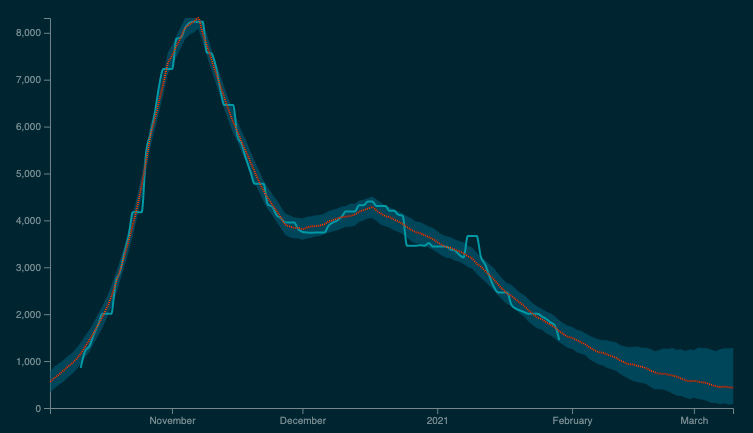
\includegraphics[scale=.328]{figs/screenshot-prediction.png}}
\caption{The visualization generated after creating a prediction model. We can see the prediction knows about a saturating minimum of zero and approximates this number slowly when predicting into the future. Blue line: the actual time series used to fit the model. Red line: \(yHat\). Blue area: uncertainty interval.}
\label{fig:screenshot-prediction}
\end{figure}

The model can then be fitted with Stan \cite{b5} specifying the distributions to sample from for the different parameters. The user choosing the prior variables is supported by our boundary visualizations that show the effects of the latest changes to their model as seen in Figure \ref{fig:screenshot-prediction}.

\subsection{Analyst-in-the-Loop Modeling}

The user, our analyst, is in the loop while modeling and can define a set of parameters to introduce their knowledge to receive a reliable and high-quality model.

\begin{itemize}
    \item \textbf{Change points:} Known dates of change points, such as dates of governments putting measures into place, can be directly specified.
    \item \textbf{Holidays and seasonality:} Users can enable country holidays for the model to learn these effects.
    \item \textbf{Smoothing parameters:} By adjusting the smoothing parameter a user can select from within a range of more global or locally smooth models. The seasonality and holiday smoothing parameters allow the user to tell the model how much of the historical seasonal variation is expected in the future.
\end{itemize}

We don't provide component charts to the users yet, where trend, seasonality, and holiday effects can be inspected individually. This would be a helpful future improvement to understand what effect the latest parameter change yielded in exactly. 

The full list of hyper parameters can be seen in table \ref{tab:hyper-params}.

\begin{table*}
  \caption{Hyper Parameter List}
  \centering
  \begin{tabular}{|p{3.5cm}||p{1.6cm}|p{1.6cm}|p{9.6cm}|} % must sum to 16.3cm
     \hline
     Parameter & Default Value & Customizable & Comments\\
     \hline
     \hline
     $growth$                    & logistic         & no  & The other option $linear$ does not respect caps or floors, and thus would produce invalid forecasts. We specify a cap of \(max(df) * 10\) to ensure we have enough head room and not run into integer overflow problems. \\
     \hline
     $changepoints$              & auto detection & yes & This is a list of customizable change points, if the user wants to define it themselves. If this is empty, we use the setting of $n\_changepoints$ to auto detect change points. \\
     \hline
     $n\_changepoints$           & 25             & yes & The number of change points of 25, should likely fit COVID-19 data. If the user selects a short time frame or want to apply regularization, they might want to reduce this number. \\
     \hline
     $changepoint\_range$        & 0.9            & yes & The model will use this percentage range to detect change points and will not place any in the remaining data. E.g., a trend change in the last 10\% will likely produce a bad forecast. We increased this number from 0.8 which was recommended by the authors of Prophet to allow the model to cope with all the measures put into place against COVID-19 and also produce slightly wider uncertainty bounds, which does not lead users into taking the prediction too seriously.  \\
     \hline
     $yearly\_seasonality$       & off            & no  & Our data barely covers a year, and certainly we need to wait several years until we could try and find yearly seasonality. For that to work, the virus must also stick around quite a while, which we all hope it will not. \\
     \hline
     $weekly\_seasonality$       & auto           & no  & We know COVID-19 data has a pretty strong weekly seasonality. So, we leave this on auto. \\
     \hline
     $daily\_seasonality$        & off            & no  & We don't have sub-daily data, so we turn it off. \\
     \hline
     $holidays$                  & off            & yes & The user is able to add the holidays of the country, read from the Python holidays library, to the model if they wish to. The effects are only marginal and do not apply yet, because holidays usually have a yearly interval, and we need more data to fully make use of this. Nonetheless it is interesting to see that the model can extract holiday effect on past data, even it cannot apply it to forecasts. \\
     \hline
     $seasonality\_mode$         & additive       & yes & This is only relevant, if the user creates forecasts without smoothing. They can change the setting to multiplicative. \\
     \hline
     $seasonality\_prior\_scale$ & 10             & yes & This parameter controls the flexibility of the seasonality. \\
     \hline
     $holidays\_prior\_scale$    & 10             & yes & This controls flexibility to fit holiday effects. \\
     \hline
     $changepoint\_prior\_scale$ & 0.5            & yes & This is probably the most impactful parameter. It determines the flexibility of the trend, and in particular how much the trend changes at the trend change points. The authors of Prophet recommend a default value of 0.05, but we change this default to be 0.25 for our use case. The trend changes in the past have been pretty strong, as measures put into place actually have their desired effect and turn around curves 90°. This fact also reveals that our predictions will not be "that" good. \\
     \hline
     $mcmc\_samples$             & off            & no  & We disable Monte Carlo sampling which can be used to not only get uncertainty in trend, but also the uncertainty in seasonality. Most of the time we are not interested in seasonal effects when creating forecasts for COVID-19 data. It also uses a lot more compute resources than Maximum a posteriori (MAP) estimation (which we use instead). \\
     \hline
     $interval\_width$           & 0.8            & no  & This is the percentage width of the uncertainty interval. We decided that this parameter is not customizable, since it doesn't change the prediction, only how it is visualized. This parameter makes sense if you use Prophet to do anomaly detection, whereas you can tune it to give you more or less anomalies according to feedback. \\
     \hline
  \end{tabular}
  \label{tab:hyper-params}
\end{table*}

\subsection{User Authentication}
To create a forecast, a user needs to be logged in to our system. They can use social identity providers such as Google or GitHub. This way they don't need to create a new account with a new password to remember.

We require users to be authenticated, so we can associate a generated prediction to a person. This lets users find their models again easily, even when logged in on a different device, and solves the question of who can edit an existing model, it's the owner of the model. It also allows us to display the name of the creator next to a prediction, should a prediction model be published and made discoverable. By making clear that a prediction has been created by another user, we implicitly transmit a message to users discovering this prediction that this is not machine generated and that a person created this (albeit with a lot of help from a machine). This automatically makes users think different about a prediction. They will know that humans are imperfect (especially on the Internet) and produce results that might be inaccurate or unusable. If we would provide predictions to all users by the system, they might fall into a false sense of certainty, that this forecast must be true, and might make conclusions that are dangerous for themselves or others. 
